% Figure 3: Pool comparison — puzzle type distributions, Hunt 1 vs Hunt 2
% Uses pgfplots + subcaption. Self-contained figure environment.
% Puzzle types listed in Hunt-1-descending order on both charts for direct comparison.
% Visual/spatial bars are starred ($\bigstar$) as the only type at comparable frequency.

\begin{figure*}[t]
\centering

% -----------------------------------------------------------------------
% Shared y-axis order (Hunt 1 descending, then Hunt-2-only types appended)
%   1 Knowledge extraction  (H1:4, H2:2)
%   2 Visual/spatial        (H1:3, H2:2)  ← comparable; starred
%   3 Logic grid            (H1:2, H2:3)
%   4 Word transformation   (H1:2, H2:3)
%   5 Cryptic               (H1:2, H2:0)
%   6 Other/mixed           (H1:2, H2:0)
%   7 Chain-following       (H1:0, H2:3)
%   8 Matching              (H1:0, H2:2)
% -----------------------------------------------------------------------

\begin{subfigure}[t]{0.47\linewidth}
  \centering
  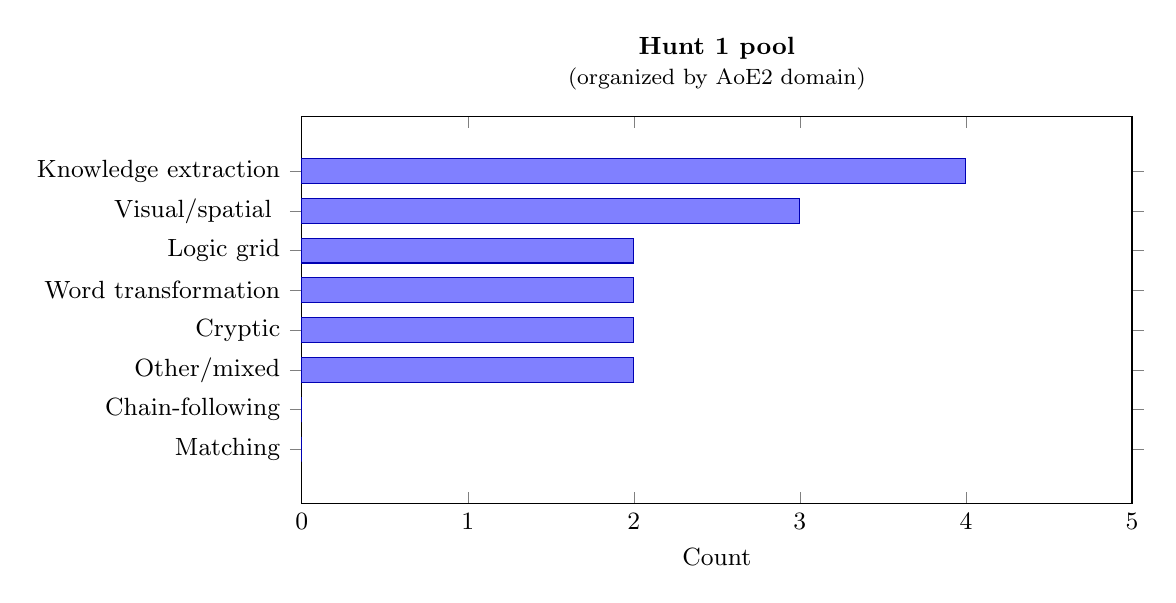
\begin{tikzpicture}
    \begin{axis}[
      xbar,                          % horizontal bars
      xmin=0, xmax=5,
      xtick={0,1,2,3,4,5},
      xlabel={Count},
      ytick={1,2,3,4,5,6,7,8},
      yticklabels={%
        Knowledge extraction,
        Visual/spatial $\bigstar$,
        Logic grid,
        Word transformation,
        Cryptic,
        Other/mixed,
        Chain-following,
        Matching%
      },
      ymin=0.3, ymax=8.7,
      y dir=reverse,                 % top-to-bottom descending
      tick label style={font=\small},
      xlabel style={font=\small},
      title={\textbf{Hunt~1 pool}\\{\footnotesize(organized by AoE2 domain)}},
      title style={align=center, font=\small},
      bar width=9pt,
      enlarge y limits=0.08,
      width=\linewidth,
      height=6.5cm,
      clip=false,
      % zero bars still draw axis line
    ]
      % Hunt 1 data (type index, count)
      \addplot[
        xbar,
        fill=blue!50,
        draw=blue!70!black,
      ] coordinates {
        (4,1)   % Knowledge extraction
        (3,2)   % Visual/spatial
        (2,3)   % Logic grid
        (2,4)   % Word transformation
        (2,5)   % Cryptic
        (2,6)   % Other/mixed
        (0,7)   % Chain-following (absent)
        (0,8)   % Matching (absent)
      };
    \end{axis}
  \end{tikzpicture}
  \caption*{}% blank; shared caption below
\end{subfigure}
\hfill
\begin{subfigure}[t]{0.47\linewidth}
  \centering
  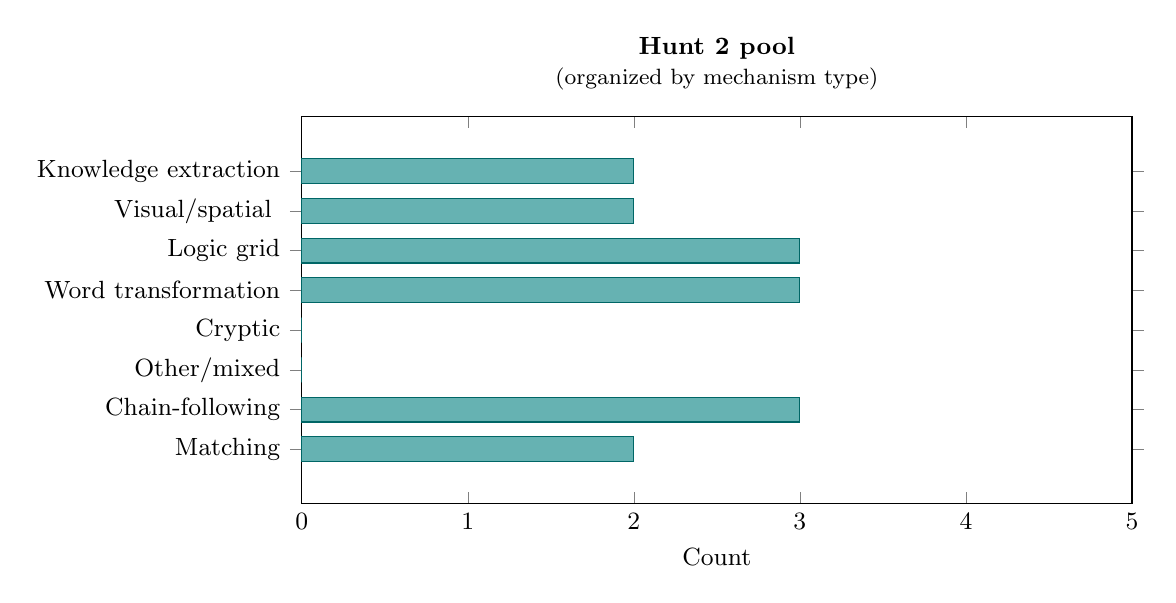
\begin{tikzpicture}
    \begin{axis}[
      xbar,
      xmin=0, xmax=5,
      xtick={0,1,2,3,4,5},
      xlabel={Count},
      ytick={1,2,3,4,5,6,7,8},
      yticklabels={%
        Knowledge extraction,
        Visual/spatial $\bigstar$,
        Logic grid,
        Word transformation,
        Cryptic,
        Other/mixed,
        Chain-following,
        Matching%
      },
      ymin=0.3, ymax=8.7,
      y dir=reverse,
      tick label style={font=\small},
      xlabel style={font=\small},
      title={\textbf{Hunt~2 pool}\\{\footnotesize(organized by mechanism type)}},
      title style={align=center, font=\small},
      bar width=9pt,
      enlarge y limits=0.08,
      width=\linewidth,
      height=6.5cm,
      clip=false,
    ]
      % Hunt 2 data
      \addplot[
        xbar,
        fill=teal!60,
        draw=teal!80!black,
      ] coordinates {
        (2,1)   % Knowledge extraction
        (2,2)   % Visual/spatial
        (3,3)   % Logic grid
        (3,4)   % Word transformation
        (0,5)   % Cryptic (absent)
        (0,6)   % Other/mixed (absent)
        (3,7)   % Chain-following
        (2,8)   % Matching
      };
    \end{axis}
  \end{tikzpicture}
  \caption*{}
\end{subfigure}

% -----------------------------------------------------------------------
% Summary annotation row
% -----------------------------------------------------------------------
\vspace{2pt}
\noindent\hfill
\begin{minipage}{0.92\linewidth}
  \centering
  \small
  \setlength{\tabcolsep}{10pt}
  \begin{tabular}{ll}
    \textbf{Type-distribution Jaccard:} & $0.11$ \\
    \textbf{Shared types at equal frequency:} & 1 of 6 represented types
      (Visual/spatial, count\,=\,2 in both pools;\;$\bigstar$)
  \end{tabular}
\end{minipage}
\hfill\null
\vspace{4pt}

\caption{Puzzle type distributions in the Hunt~1 pool (left, organized by AoE2
  domain) and Hunt~2 pool (right, organized by mechanism type). Despite
  identical domain inputs, the pools organized around different structural
  principles, producing minimal type overlap (Jaccard\,=\,0.11).
  Visual/spatial is the only type represented at comparable frequency in
  both pools~($\bigstar$).}
\label{fig:pools}
\end{figure*}
